\chapter{Proposed Method}
\label{chapter:method}


\section{Compositional Class label-to-Image Diffusion model (CCDM)}
\label{sec:CCDM}
Our model is a diffusion model conditioned on a compositional class label $c$, where $c = [c_1, \dots, c_n]$ is composed of a combination of labels from different categories. We use $n = 2$ and $n = 3$(two conditions and three conditions) for our model. In this chapter, we further decomposed our model into several components to introduce our approach: the denoising model , the conditioning module, and the compositional class encoder. As mentioned in Section \ref{sec:ddpm}, the denoising model is used to predict noise based on a compositional class label $c$, a timestep $t$ and a noisy sample $x_t$, with this model, we can use Eq. \ref{eq:14} to restore $x_t$ to $x_0$. The conditioning module is how we add conditional information into our denoising model, we employ four different architectures to integrate the information of compositional class labels.
The compositional class encoder is used to encode the compositional class label $c$, mapping the class label to a higher-dimensional space.
\begin{figure} [H]
    \centering
    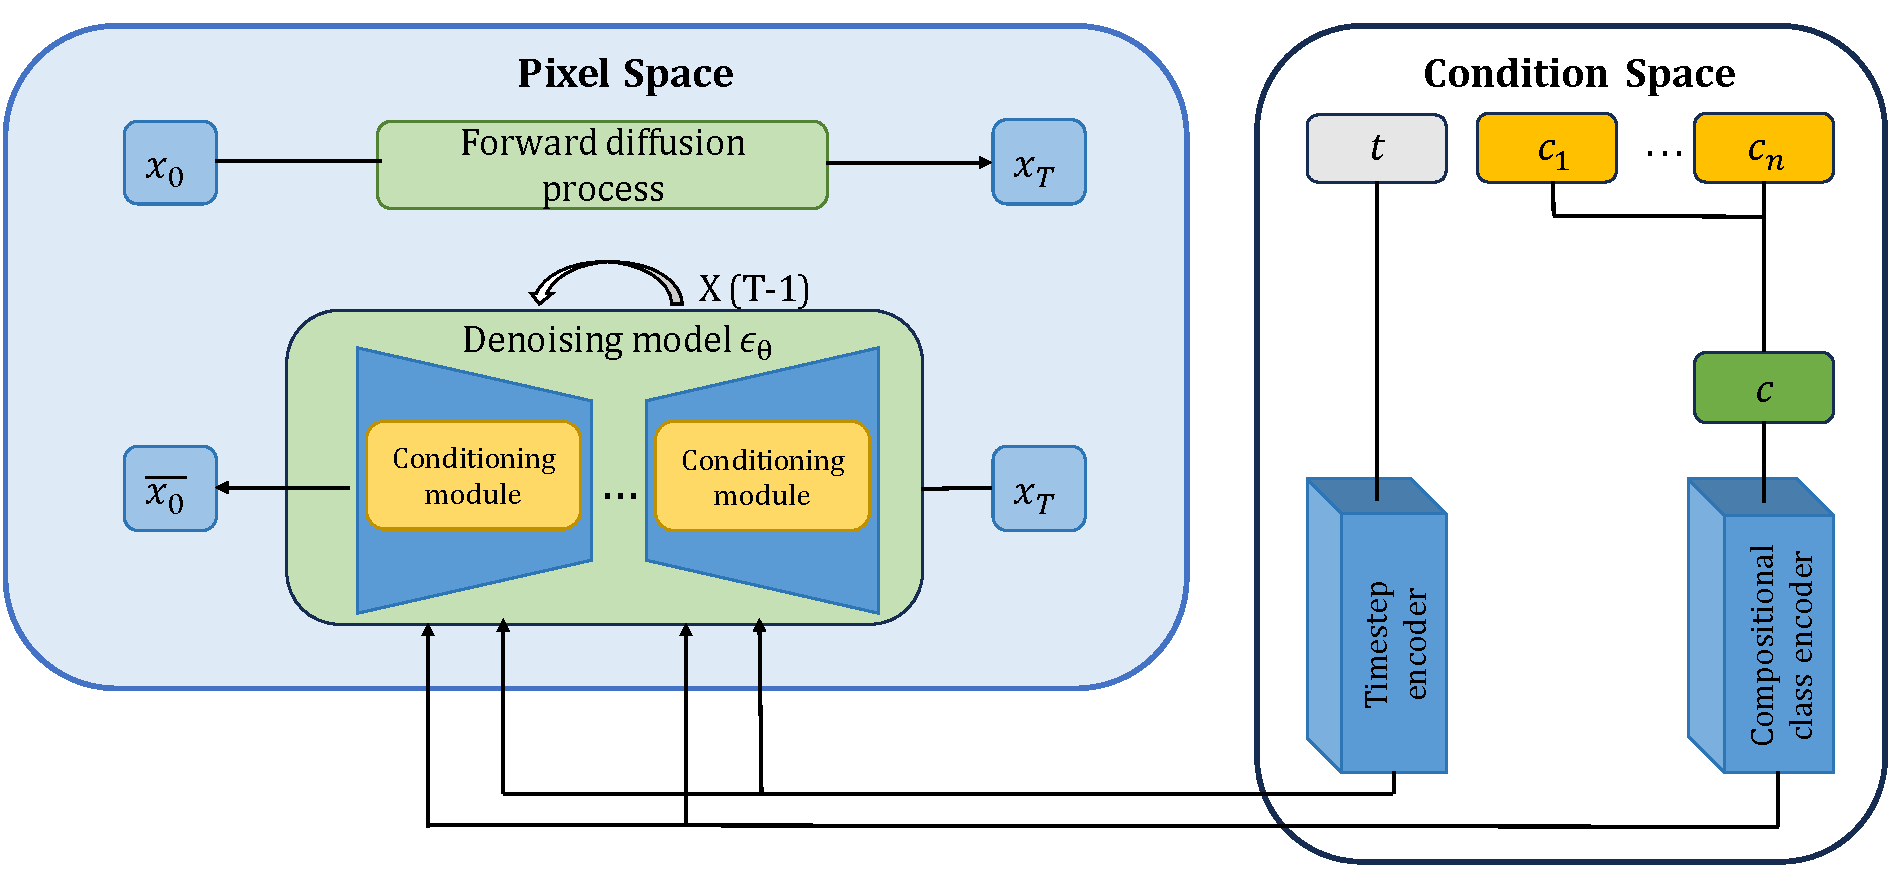
\includegraphics[width=0.8\linewidth]{figures/CCDMBlock.pdf}
    \caption{Block diagram of CCDM}
    \label{fig:CCDM}
\end{figure}
Figure \ref{fig:CCDM} illustrates the architecture of our model, the compositional class label will be encoded by the class encoder and integrate with the conditioned denoising model through the conditioner, and the conditioned denoising model will predict the noise term based on conditional information.

\section{Compositional class encoder}
In order to guide the diffusion model with compositional class information, we first use one-hot encoding to encode the compositional class label for different categories. Given $c = (c_1, c_2, c_3, ...)$ is the compositional class label, the compositional class encoder is illustrated as the follows:
\begin{figure} [H]
    \centering
    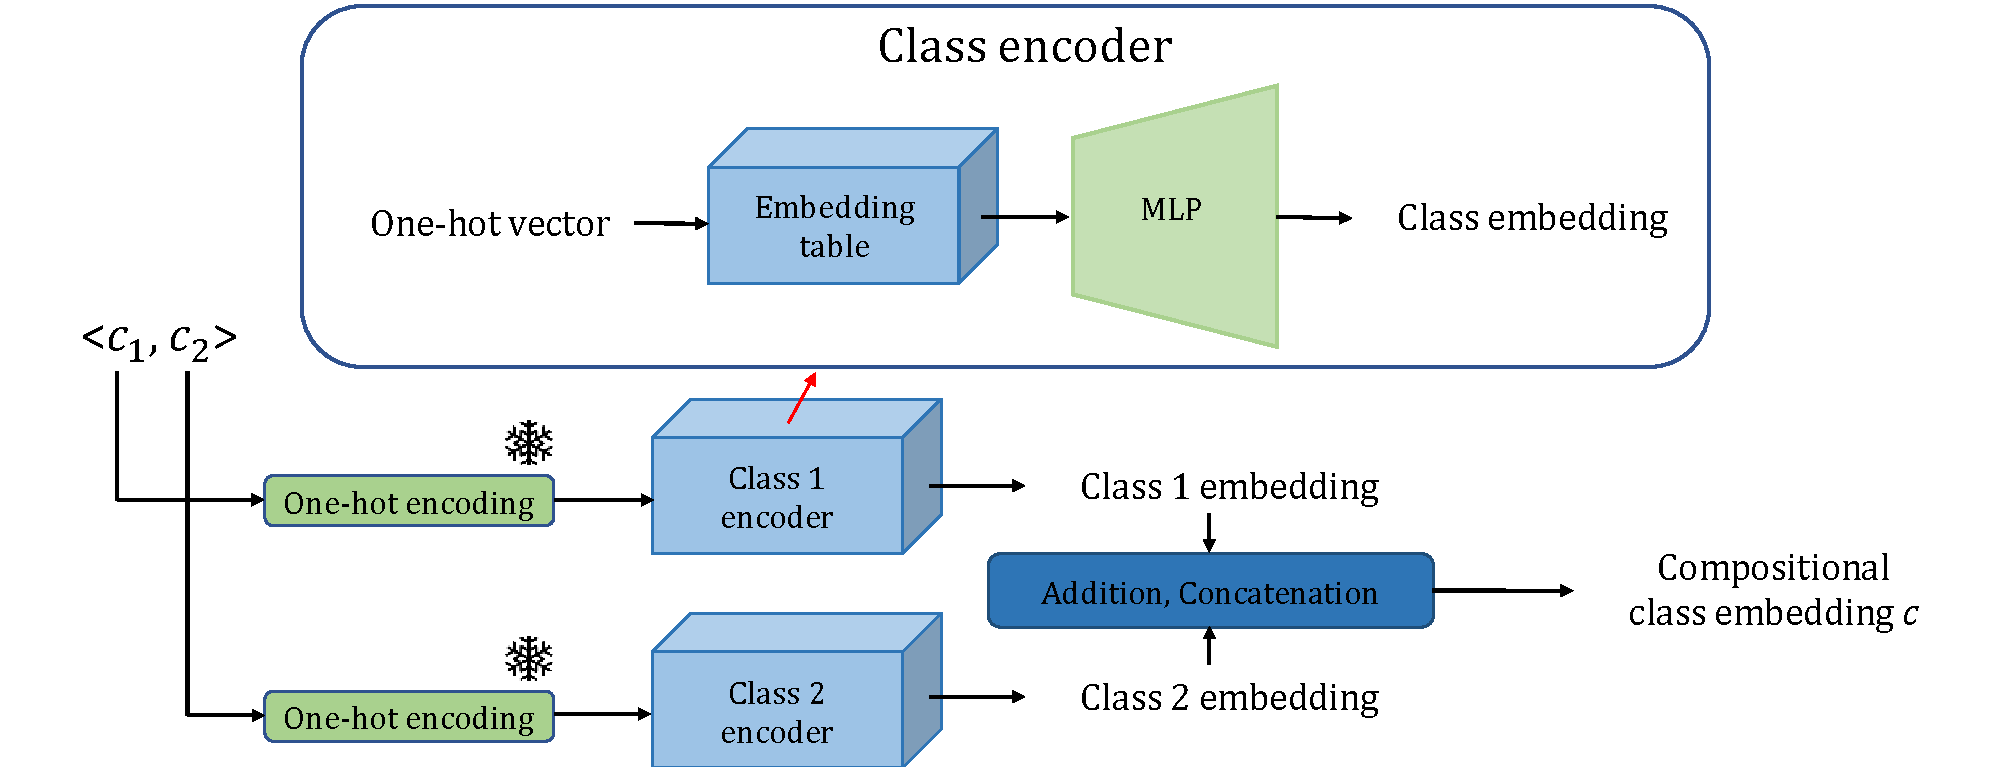
\includegraphics[width=1\linewidth]{figures/Class encoder.pdf}
    \caption{Compositional class encoder}
    \label{fig:class encoder}
\end{figure}

For each category's class label, we first encode them using one-hot encoding. Then, we use an embedding table and MLP to encode the one-hot vector. Finally, we sum or concatenate these class embeddings based on different conditioning modules. Figure \ref{fig:class encoder} illustrates how we encode compositional class labels using two category class labels.

\section{Denoising model}
According to Chapter \ref{chapter:preliminary}, we added a compositional class label $c$ to guide our denoising model. We modify Eq.\ref{eq:10} to cooperate with compositional class label $c$ and sampled image according to the compositional label $c$. The modified loss function will be:
\begin{equation}
    L_{simple} = \mathbb{E}_{x_0, \epsilon}[\|\epsilon - \epsilon_\theta(\sqrt{\overline{\alpha}_t}x_0 + \sqrt{1 - \overline{\alpha}_t}\epsilon, t, c)\|^2]
\end{equation}
Our denoising model $\epsilon_\theta$ now has three inputs, which are the noisy sample $x_t$, timestep $t$ and the compositional label $c$ instead of only $x_t$ and $t$. The training and sampling procedure are illustrated as the follows:
\begin{algorithm}
\caption{Training CCDM}
\label{training}
\vspace{2mm}
\begin{algorithmic}[1]
\Repeat: \vspace{2mm}
    \State $(x_0, c) \sim p(x, c)$  \vspace{2mm}
    \State $c \leftarrow \varnothing \text{ with probability } p_{uncond}$
    \State $t \sim Uniform(\{1, \dots, T\})$ \vspace{2mm}
    \State $\epsilon \sim \mathcal{N}(0, \textbf{I})$ \vspace{2mm}
    \State $x_t = \sqrt{\overline{\alpha}_t}x_0 + \sqrt{1 - \overline{\alpha}_t}\epsilon$ \vspace{2mm}
    \State Take a gradient step on $ \nabla_{\theta} \| \epsilon - \epsilon_\theta(\sqrt{\overline{\alpha}_t}x_0 + \sqrt{1 - \overline{\alpha}_t}\epsilon, t, c) \|^2 $ \vspace{2mm}
    \Until converged \vspace{2mm}
\end{algorithmic}
\end{algorithm}

\begin{algorithm}
\caption{Sampling}
\label{sampling}
\vspace{2mm}
\begin{algorithmic}[1]
\Require $\omega:$ guidance scale \vspace{2mm}
\Require $c:$ Compositional class label for compositional generation
\Require $\eta:$ hyperparameter controlling sampling stochasticity \vspace{2mm}
\State $x_t \sim \mathcal{N}(0, \textbf{I})$ \vspace{2mm}
\For{t = $S, \dots, 1$} \vspace{2mm}
    \State $\epsilon \sim \mathcal{N}(0, \textbf{I})$ if $t > 1$, else $\epsilon = 0$ \vspace{2mm}
    \State $\sigma_t = \eta \cdot \tilde{\beta}_t$ \vspace{2mm}
    \State $\tilde{\epsilon}_t = (1 + \omega)\underbrace{\epsilon_\theta(x_t, t, c)}_{\text{conditional noise}} - \omega\underbrace{\epsilon_\theta(x_t, t, \varnothing)}_{\text{unconditional noise}}$ \vspace{4mm}
    \State $x_{t-1} = \sqrt{\alpha_{t-1}}(\frac{x_t - \sqrt{1 - \alpha_t}\tilde{\epsilon}_t}{\sqrt{\alpha_t}}) + \sqrt{1 - \alpha_{t-1} - \sigma_t^2} \cdot \tilde{\epsilon}_t + \sigma_t\epsilon_t$ \vspace{2mm}
\EndFor \vspace{2mm}
\State \textbf{return} $\overline{x_0}$ \vspace{2mm}
\end{algorithmic} 
\end{algorithm}

\begin{figure} [H]
    \centering
    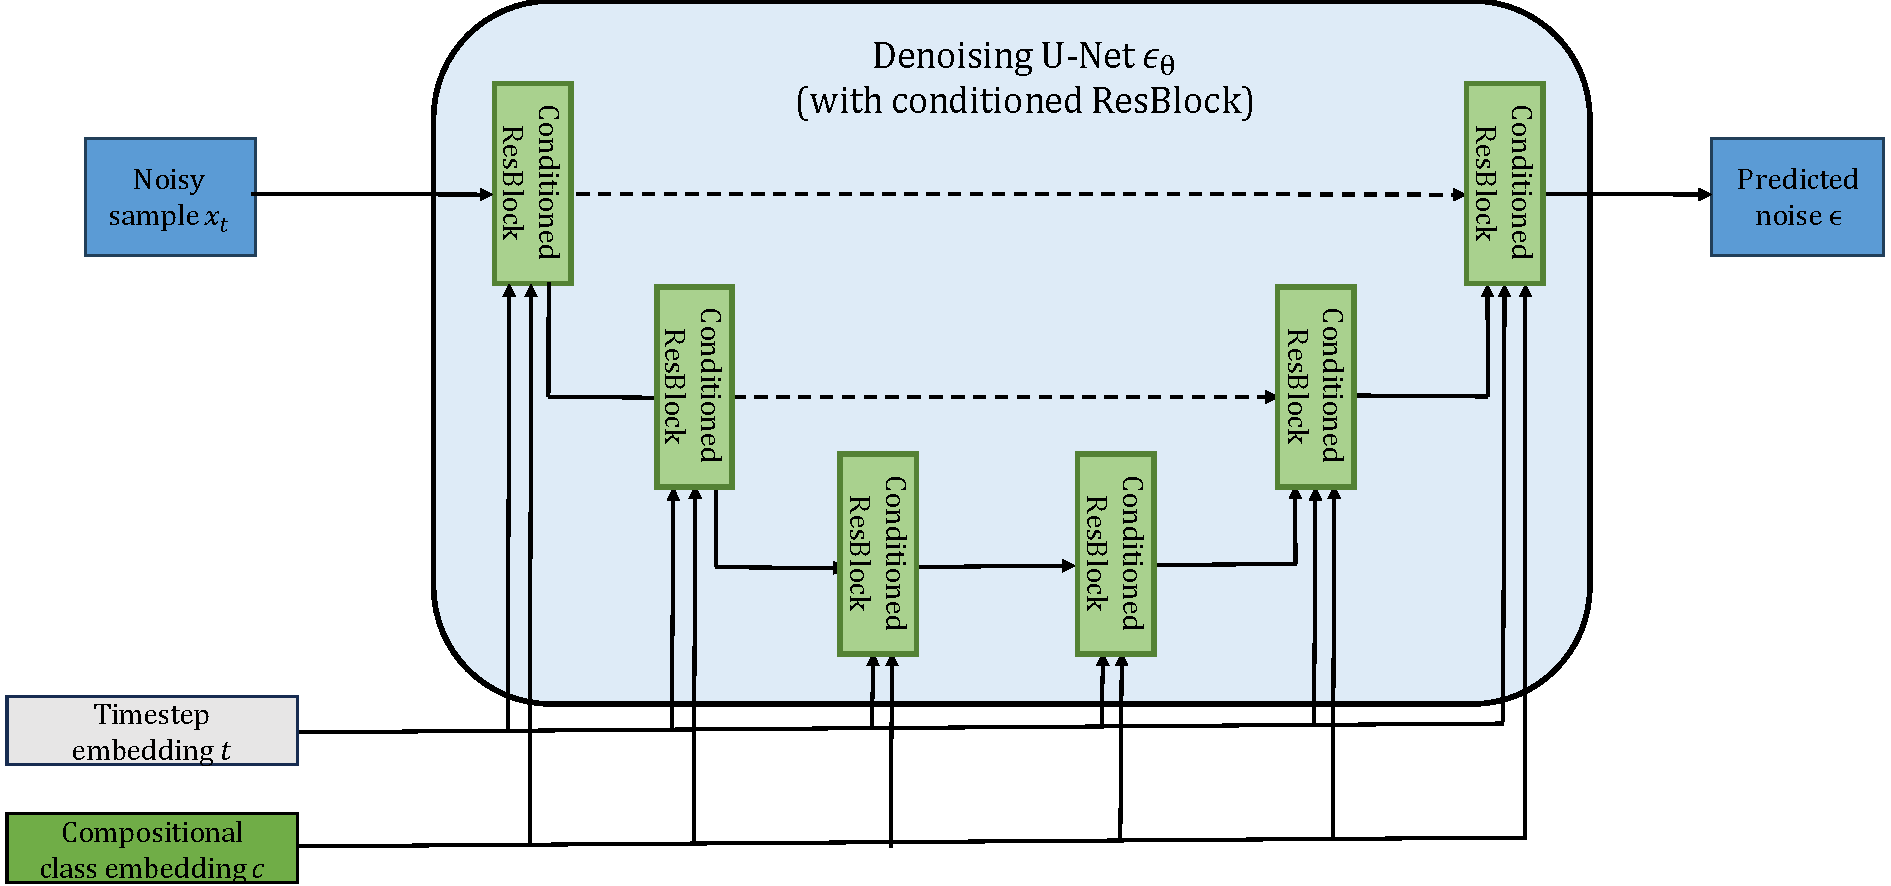
\includegraphics[width=1\linewidth]{figures/UNetRes.pdf}
    \caption{Conditioned denoising U-Net with conditioned ResBlock}
    \label{fig:unetres}
\end{figure}

\begin{figure} [H]
    \centering
    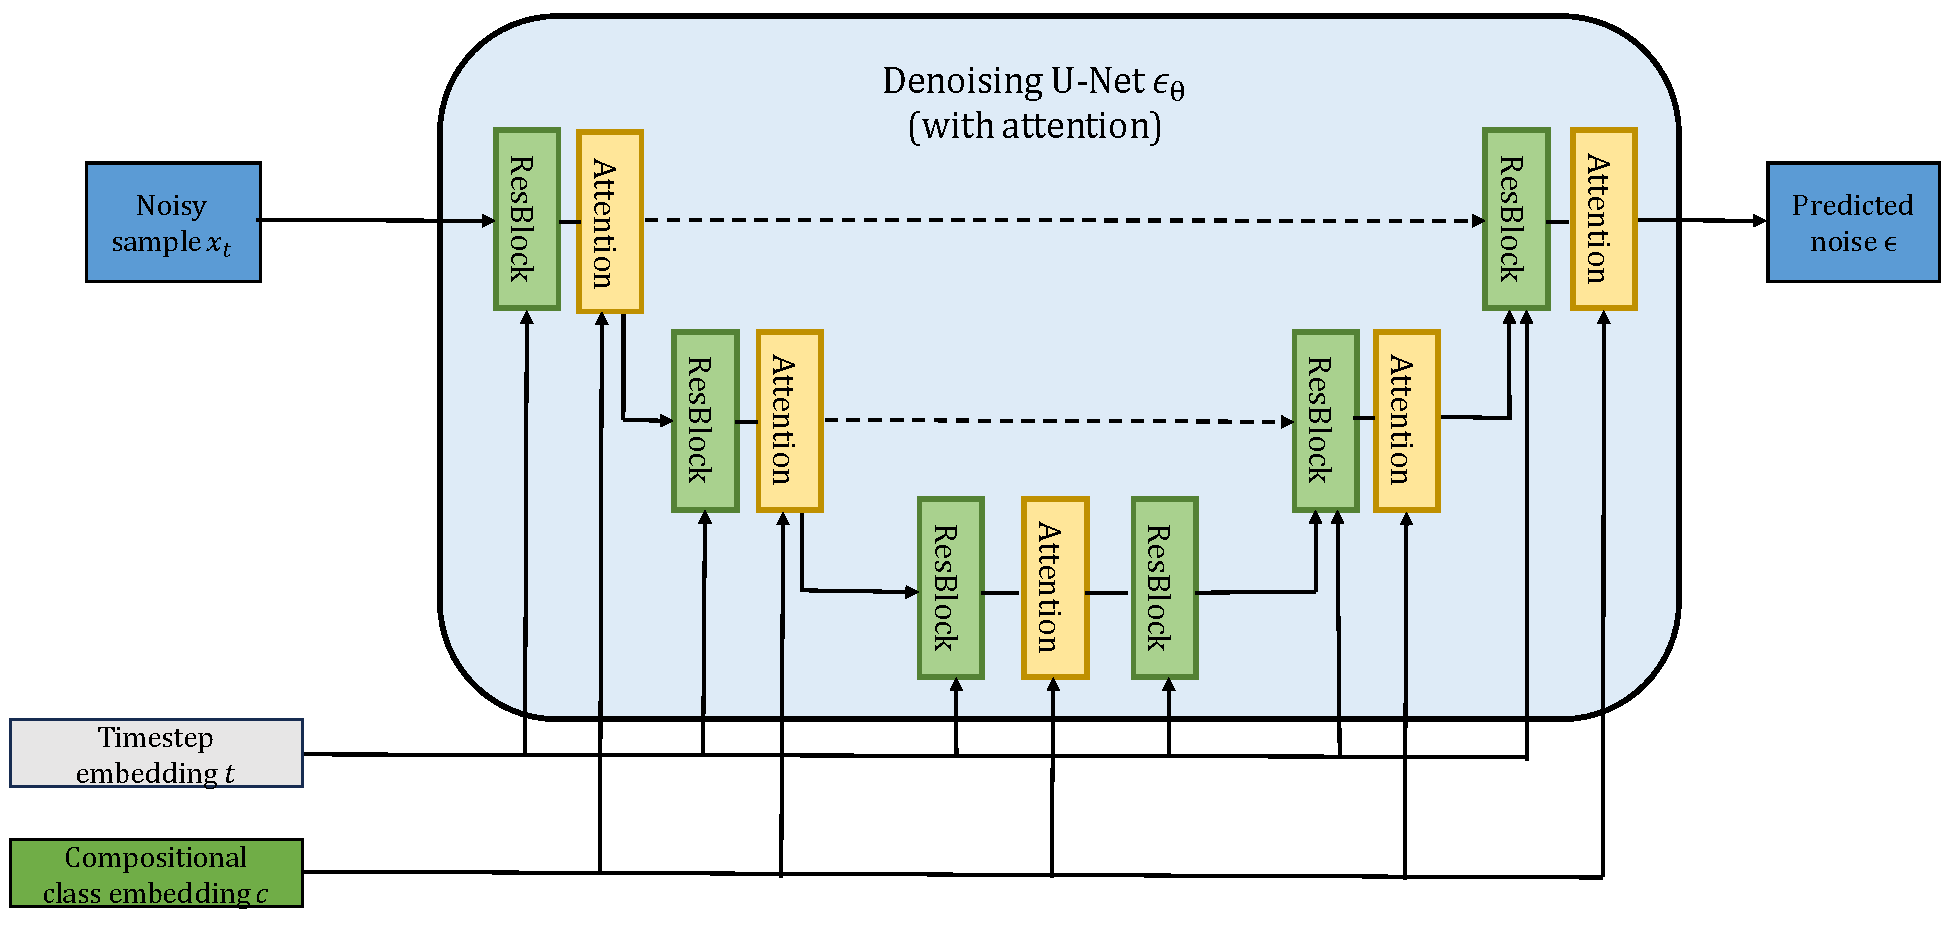
\includegraphics[width=1\linewidth]{figures/UNetAttention.pdf}
    \caption{Conditioned denoising U-Net with attention}
    \label{fig:unetattention}
\end{figure}


Figure \ref{fig:unetres} and figure \ref{fig:unetattention} shows how to integrate conditional information with each residual block in the conditioned denoising U-Net. The difference between these two U-Net architectures lies in the location where condition information is incorporated.

\section{Conditioning module}
\label{subsec: conditioning module}
There are various methods to incorporate conditional information into the denoising model. Drawing inspiration from numerous papers, we implemented four different conditioning modules in our model. In the following schematic diagram, we will illustrate how we use the information from compositional class labels to guide our model. Before introducing these conditioning modules, we need to establish definitions for some symbols. Let $h$ be the hidden state, $t$ be the timestep embedding vector, $c$ be the compositional class embedding vector and $proj$ be the linear projection layer.
\subsection{Addition (Add)}
Follow DDPM\cite{ho2020denoising} implementation, we preform element-wise addition on projected timestep embedding and compositional class embeddings into each residual block. We define the conditioning module as Add$(h, t, c)$, then
\begin{equation}
    \text{Add}(h, t, c) = h + proj(t) + proj(c)
\end{equation}

\begin{figure} [H]
    \centering
    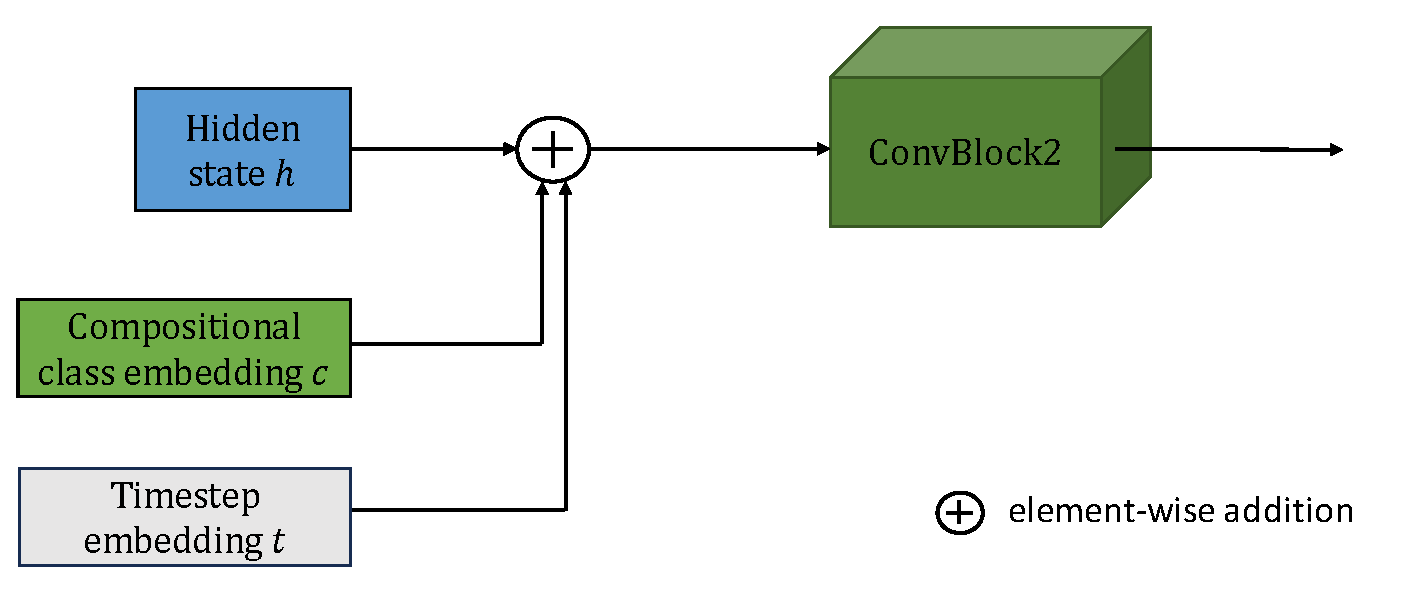
\includegraphics[width=0.8\linewidth]{figures/Add.pdf}
    \caption{Addition}
    \label{fig:add}
\end{figure}
Figure \ref{fig:add} shows how we integrate hidden state $h$ and conditional information. In each residual block, we add projected timestep embedding and projected compositional class embedding into $h$, where $h$ is the output of the first convolution block. We call this conditioning module \textbf{Add} for the rest of this thesis.
\subsection{Adaptive Group Normalization (AdaGN)}
Follow \cite{nichol2021improved} implementation, we also implement this module on our model, let $y^{\prime} = proj(y + t)$ and $y^{\prime} = [y_s, y_b]$, which we split $y^{\prime}$ into two vectors with the same dimension, then the conditioning module is illustrated as the follows:
\begin{equation}
    \text{AdaGN}(h, t, c) = (1 + c_s)\text{GroupNorm}(h) + c_b
\end{equation}
\begin{figure} [H]
    \centering
    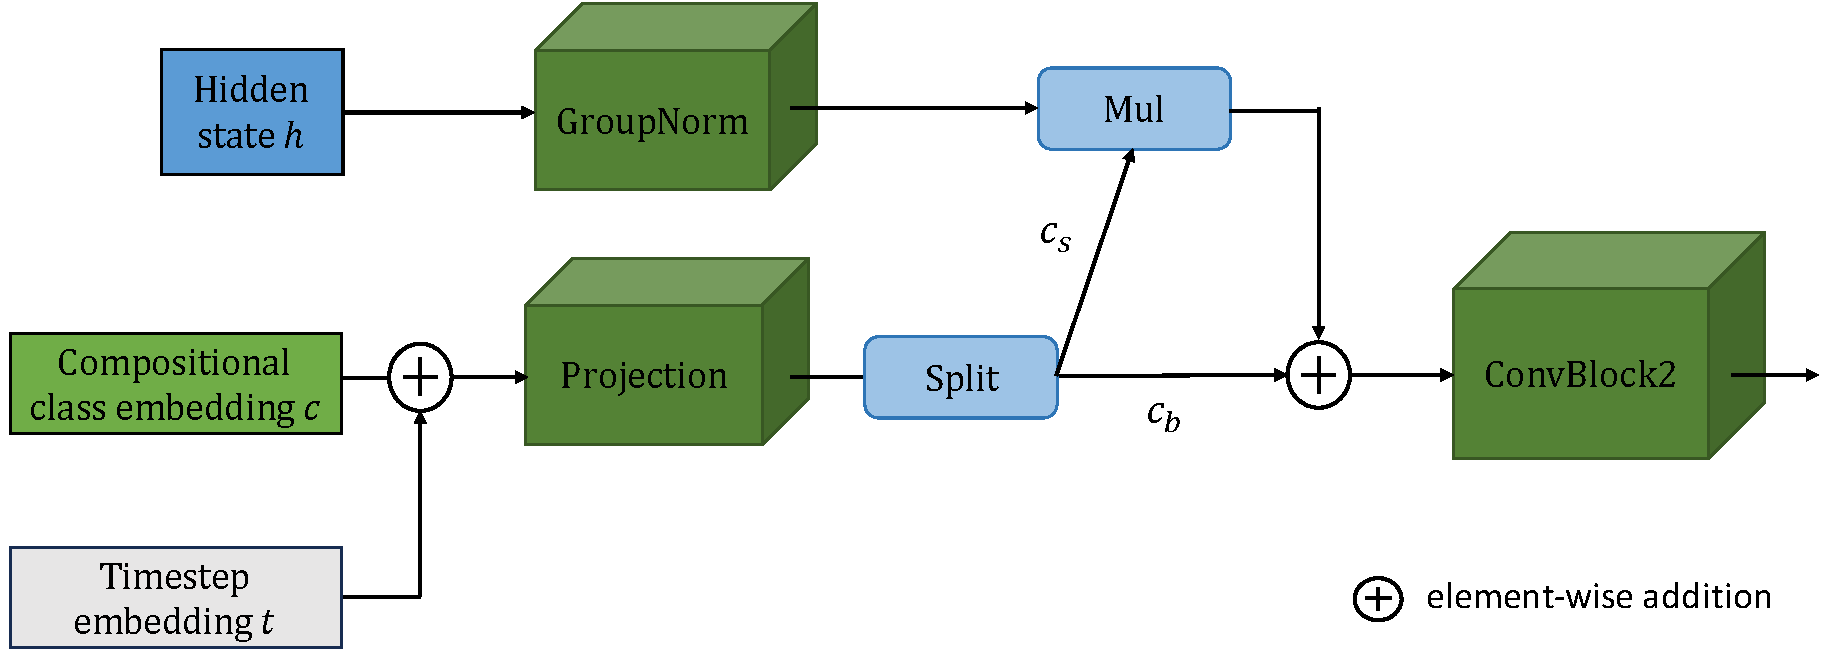
\includegraphics[width=0.8\linewidth]{figures/AdaGN.pdf}
    \caption{Adaptive Group Normalization}
    \label{fig:adagn}
\end{figure}
Figure \ref{fig:adagn} illustrates the procedure of adaptive group normalization, the projection layer maps the original dimension, which is 512, to 512 * 2, while the split operation divides the vector, originally of dimension 1024, into two 512-dimensional vectors.

\subsection{Image Class concatenation (IC)}
We concatenate compositional class embedding $y$ with hidden state $h$ to add conditional information guidance, then we use a bottleneck layer to reduce dimension after concatenation, details are illustrated as the follows:
\begin{figure} [H]
    \centering
    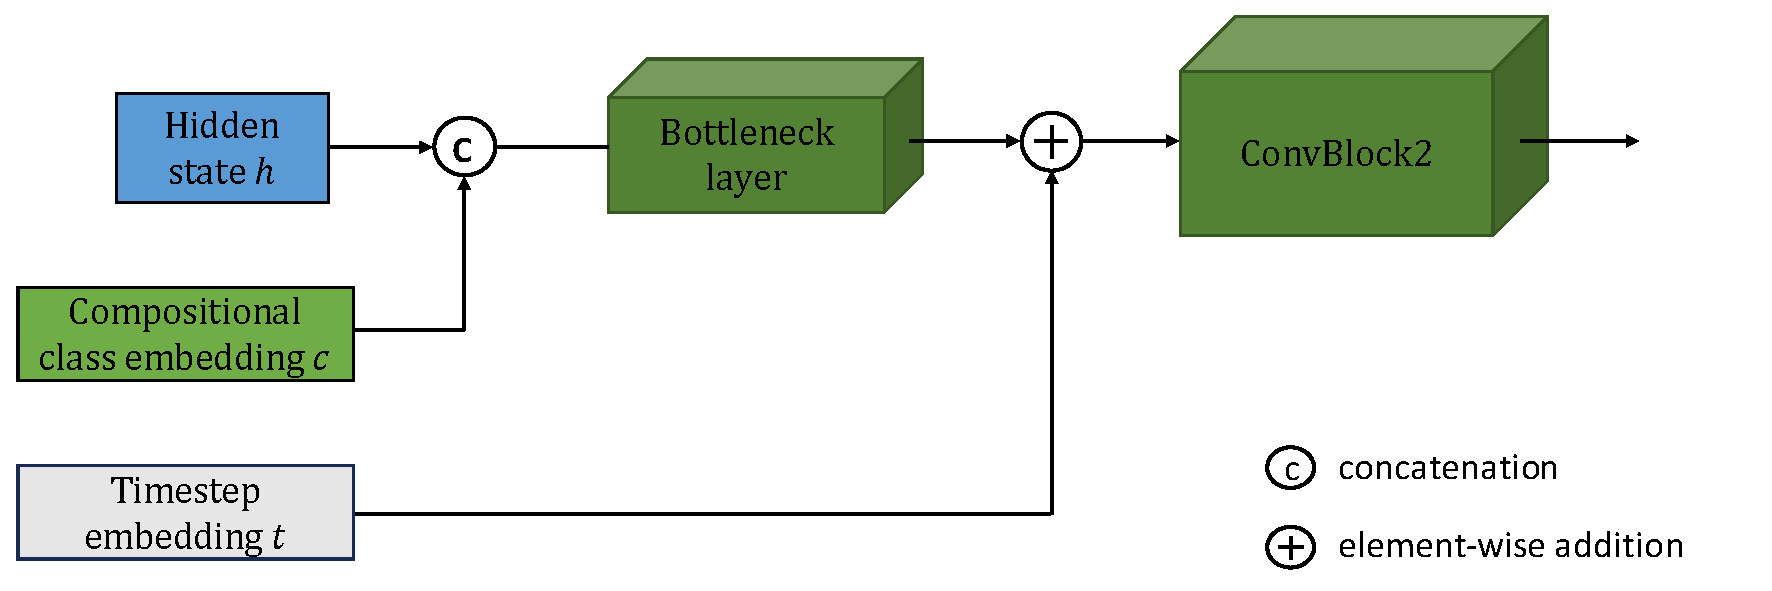
\includegraphics[width=0.8\linewidth]{figures/IC.pdf}
    \caption{Image class concatenation}
    \label{fig:ic}
\end{figure}
Follow \cite{rombach2022high} implementation of super-resolution and inpainting diffusion model. We concatenate concatenate compositional class embedding $c$ with hidden state $h$ in diffusion process.Figure \ref{fig:ic} illustrates how we integrate timestep embedding $t$ and compositional class embedding $y$ with hidden state $h$. We first combine the hidden state and compositional class information using concatenation. Then, we use a bottleneck layer for dimensionality reduction, restoring it to the original dimension. Finally, we incorporate the timestep information through element-wise addition. 

\subsection{Cross Attention (CA)}
Follow \cite{rombach2022high} implementation, we use an shallow spatial transformer composed by $N$ transformer blocks, each block consists of a multi-head self-attention layer, a position-wise feedforward network and a multi-head cross-attention layer.
\begin{figure} [H]
    \centering
    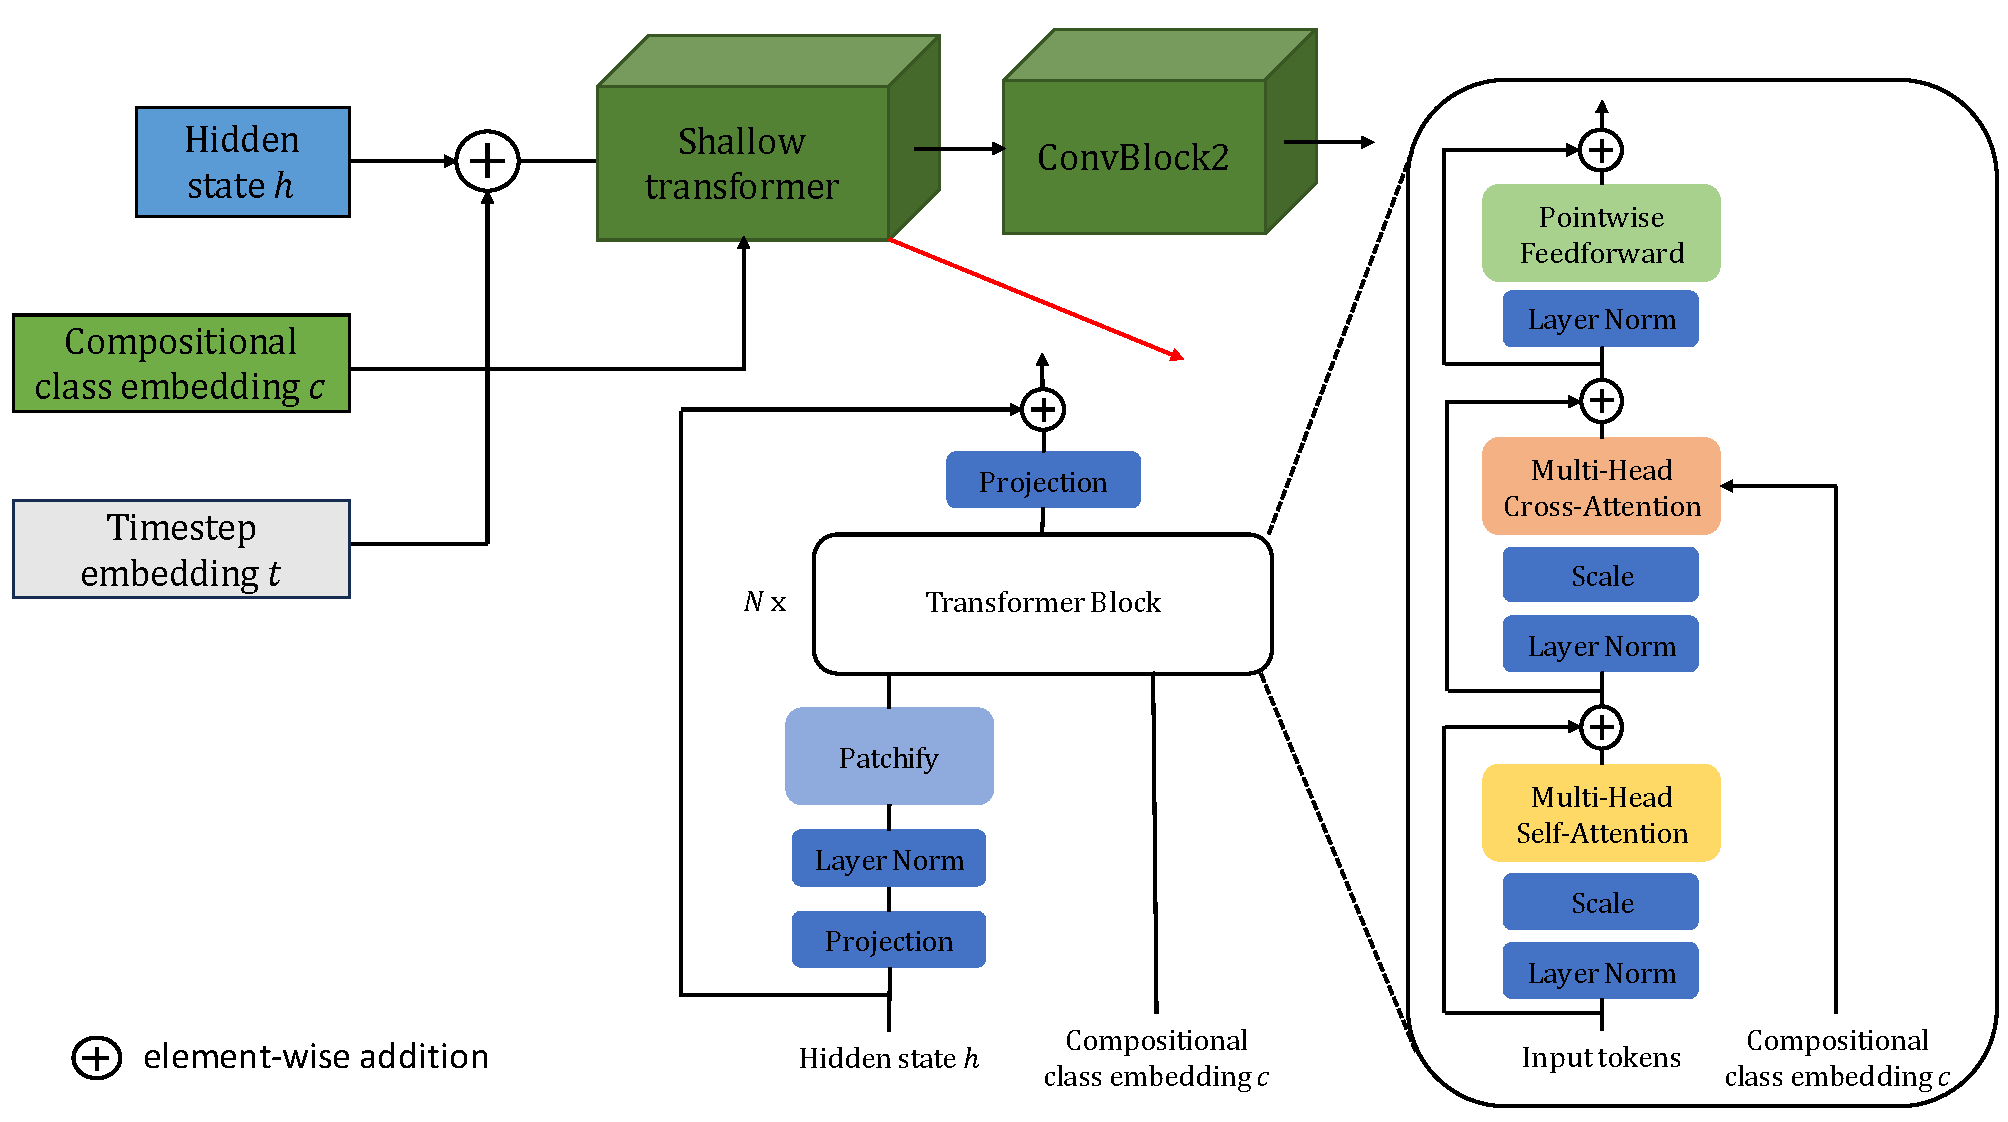
\includegraphics[width=0.8\linewidth]{figures/CA.pdf}
    \caption{Cross attention}
    \label{fig:ca}
\end{figure}
Figure \ref{fig:ca} illustrates the architecture of spatial transformer and transformer block, note that the compositional class embedding $y \in \mathbb{R}^{B \times 1 \times D_{emb}}$ is extended from the original compositional class embedding $y \in \mathbb{R}^{B \times D_{emb}}$ by adding a new dimension.

\section{Image Selector}
\label{sec:selector}
Although CCDM has the capability of compositional zero-shot image generation, not every generated image aligns perfectly with the unseen compositional class label. Sometimes, the images produced by the model may exhibit deviations. Therefore, we require a framework to assess the performance of the model.

 We introduced an image selection framework to assess the model. Following \cite{misra2017red}, we separately trained binary classifiers for the object and attribute of unseen compositions. Using ``Heel Slipper`` as an example, we would train a ``Heel`` binary classifier and a ``Slipper`` binary classifier. These classifiers are then utilized to filter the images generated by CCDM.
To ensure the reliability of these classifiers, we first generated N unseen composition images using CCDM. Subsequently, we utilized these classifiers to select images that match the unseen compositions. We then manually verified whether the selected images indeed matched the criteria.
\begin{figure} [H]
    \centering
    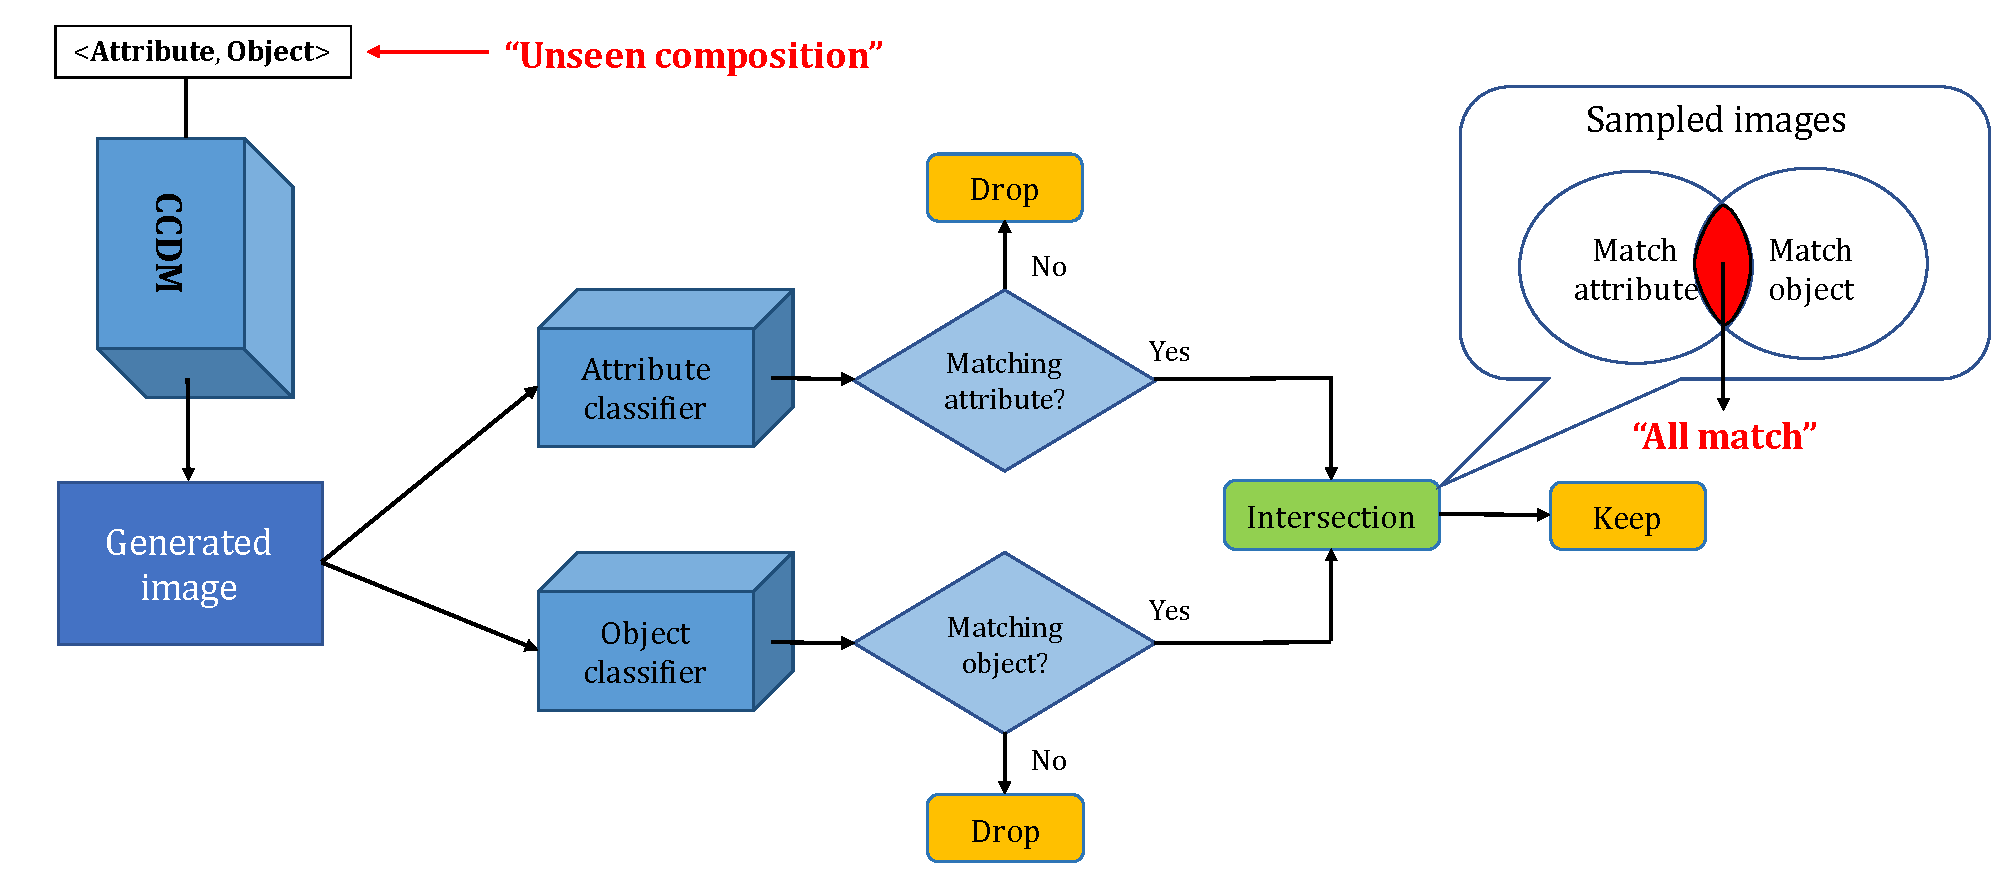
\includegraphics[width=1\linewidth]{figures/Image selector.pdf}
    \caption{Image selector on unseen composition}
    \label{fig:selection}
\end{figure}

Figure \ref{fig:selection} illustrates how we evaluate a generated image. After generating images using CCDM based on unseen compositional class labels, each generated image undergoes evaluation by multiple binary classifiers to determine whether it matches the description of the class label. 

